\section{Static Network Conditions}\label{sec:methodology}
We begin by measuring how VCAs perform under different network conditions. 
In the first set of experiments, we study the impact of \textbf{bandwidth},
and \textbf{loss} on application performance. In the second set of experiments, 
we analyze how these applications respond to new flows on the network.


\noindent\textbf{Methodology}. 
%% experiment setup
%% what is the experiment duration 
%% what bandwidth profiles are used 

\begin{center}
   \begin{figure}[]
    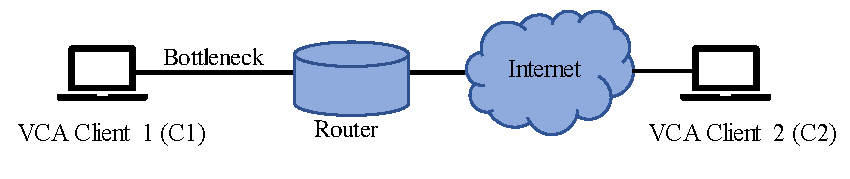
\includegraphics[width=0.45\textwidth,keepaspectratio]{../figures/methodology/normal-setup.pdf}
    \caption{Setup for static experiments}
    \label{fig:static_setup}
    \end{figure}
\end{center}

\tarun{Open questions: i) What about Team native client? ii) Audio performance? iii) Re-do \zoombrowser for 0.3 Mbps and 0.4 Mbps}

\noindent \textbf{Results}: Figure~\ref{fig:downlink_bitrate} shows the median received network bitrate averaged over 5 runs for different downlink shaping levels. We find differences among VCAs in terms of their bitrate configuration and bitrate adaptation leading to different performance under same network conditions. For instance, the peak utilization for \teamsnative is $1.9$ Mbps whereas it is only $0.8$ Mbps for \meet and $0.96$ for \zoomnative. The received bitrate also reflects how different VCAs utilize the network. We find that \zoomnative . Finally, we also notice performance differences between \teamsbrowser and \teamsnative under same network conditions. This suggests that the platform also plays an important role.  

\textbf{Network bitrate and application performance metrics}: We next analyze how network bitrate correlates with application performance metrics. We limit this analysis to only \meet, \teamschrome, and \zoomnative based on the availability of the ground truth metrics. We use WebRTC stats to obtain statistics for \teamschrome and \meet. We could not obtain the same statistics for \zoombrowser as it uses DataChannels instead of the usual MediaStream to transmit audio and video content. In addition, we also obtained access to Zoom API through our campus network operator. The Zoom API provides limited application performance at a per-second granularity.  

\textbf{Video quality vs downlink shaping level}

\textbf{}



%% zoom is able to pro

Interestingly, we find differences between \zoomnative and \zoombrowser (\tarun{re-run \zoombrowser}).

\textbf{Takeaway}: VCA performance under same network conditions varies.  
%% also plot differences in network utilization and the shaping. 



%% Difference among VCAs. Peak utlization differs. For the same network conditions, VCAs peform differently. For instance, Teams on WebRTC 
%% Difference between native and browser client 
%% Google Meet Simulcast

\begin{figure}[]
\centering
    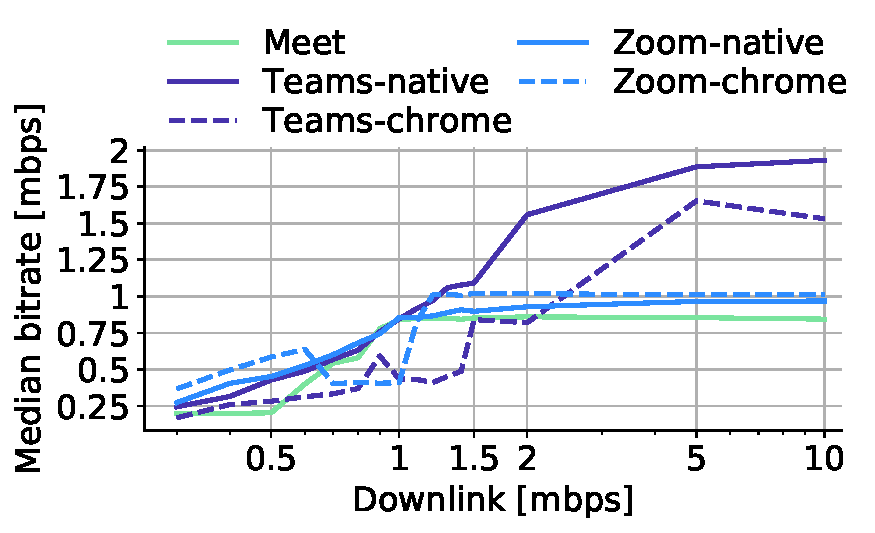
\includegraphics[width=0.35\textwidth,keepaspectratio]{figures/static/downlink.pdf}
    \caption{Downlink bandwidth vs network bitrate}
	\label{fig:downlink_bitrate}
\end{figure}



\begin{figure}[]
\centering
    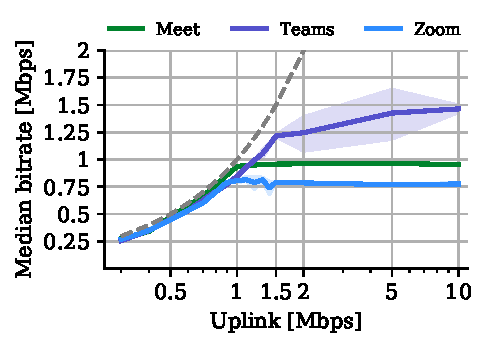
\includegraphics[width=0.35\textwidth,keepaspectratio]{figures/static/uplink.pdf}
    \caption{Uplink bandwidth vs network bitrate}
	\label{fig:uplink_bitrate}
\end{figure}




\begin{figure*}[]
	%\vspace{-1em}
    \begin{subfigure}[t]{0.3\textwidth}      
    		\centering
        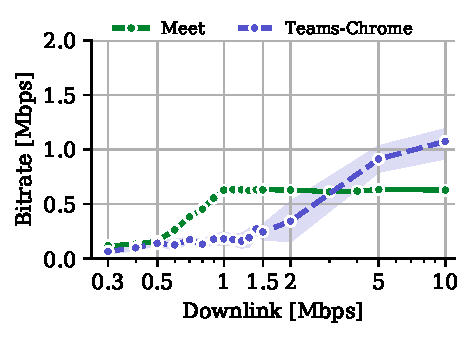
\includegraphics[width=\textwidth,keepaspectratio]{figures/static/downlink_received_bitrate.pdf}
        \vspace{-2em}
        \caption{Video bitrate}
 		\label{subfig:downlink_video_bitrate}
    \end{subfigure}%
    \hfill
	\begin{subfigure}[t]{0.3\textwidth}   
        \centering
        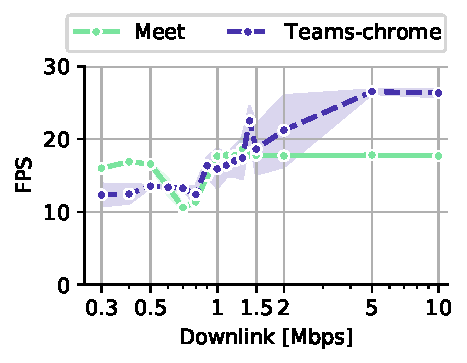
\includegraphics[width=\textwidth]{figures/static/downlink_received_framesPerSecond.pdf}
        \vspace{-2em}
    \caption{Frames per second}
    \label{subfig:downlink_frames_per_second}
    \end{subfigure}% 
    \hfill
	\begin{subfigure}[t]{0.3\textwidth}   
        \centering
        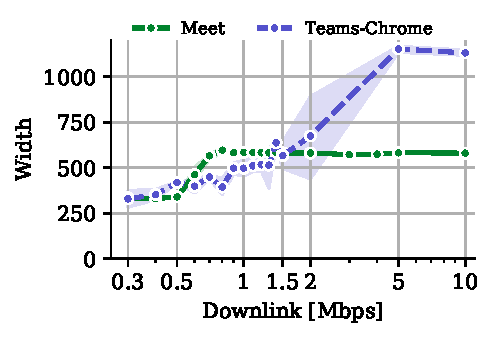
\includegraphics[width=\textwidth]{figures/static/downlink_received_frameWidth.pdf}
        \vspace{-2em}
    \caption{Frame width}
    \label{subfig:downlink_frame_width}
    \end{subfigure}
    \newline
        \begin{subfigure}[t]{0.3\textwidth}      
    		\centering
        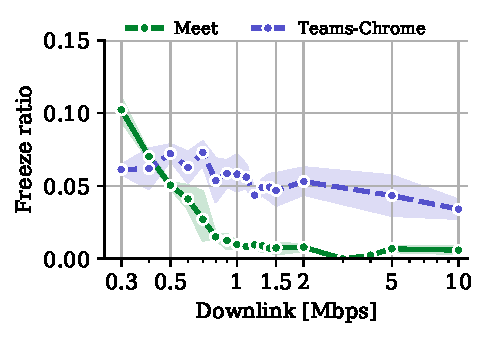
\includegraphics[width=\textwidth,keepaspectratio]{figures/static/downlink_freezeRatio.pdf}
        \vspace{-2em}
        \caption{Freeze ratio}
 		\label{subfig:downlink_freeze_ratio}
    \end{subfigure}%
    \hfill
	\begin{subfigure}[t]{0.3\textwidth}   
        \centering
        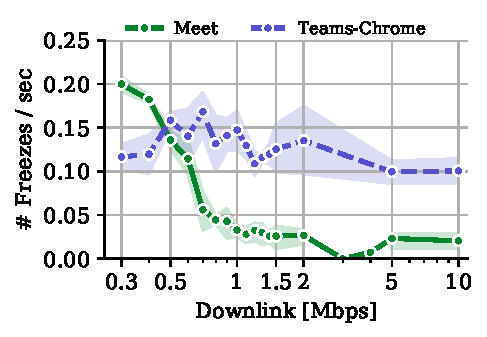
\includegraphics[width=\textwidth]{figures/static/downlink_freezeCountPerSecond.pdf}
        \vspace{-2em}
    \caption{Number of freezes per second}
    \label{subfig:downlink_freeze_per_sec}
    \end{subfigure}% 
    \hfill
	\begin{subfigure}[t]{0.3\textwidth}   
        \centering
        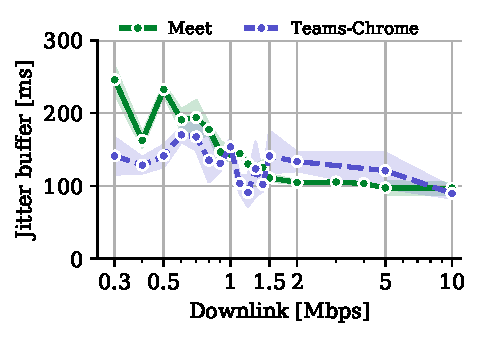
\includegraphics[width=\textwidth]{figures/static/downlink_jitter_buffer.pdf}
        \vspace{-2em}
    \caption{Jitter buffer delay}
    \label{subfig:downlink_jitter_buffer}
    \end{subfigure}
	\vspace{-1em}
	\caption{Downlink bandwidth and application performance metrics}
	\label{fig:qoe_distribution}
	%\vspace{-1em}
\end{figure*}

\begin{comment}
\begin{figure}[]
    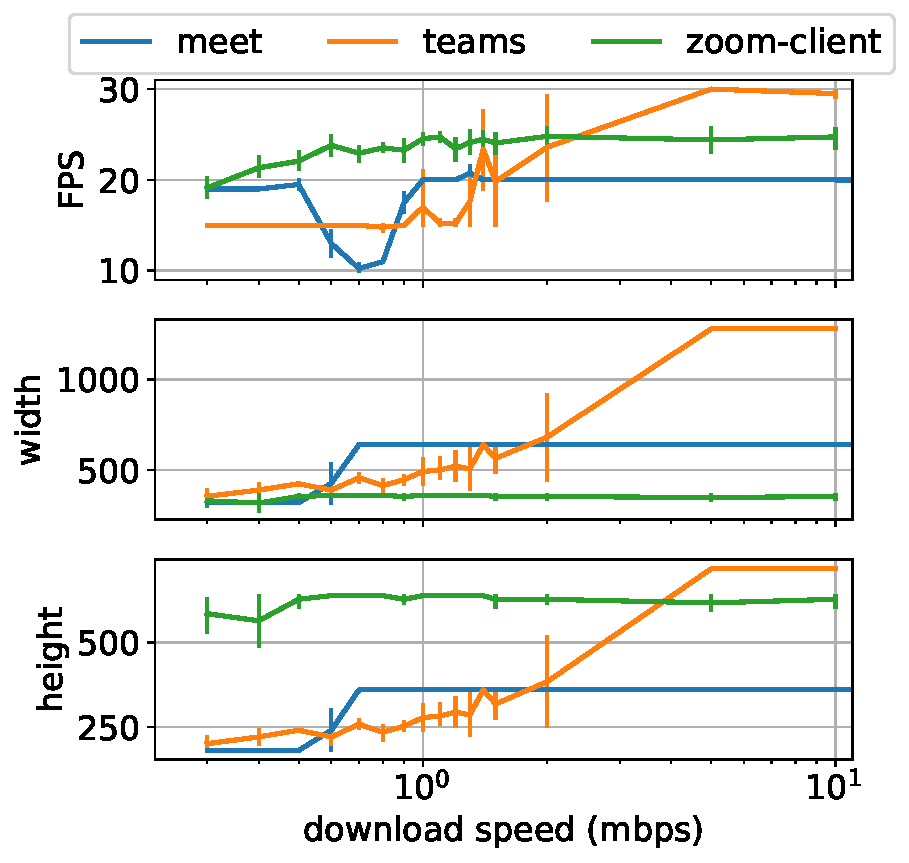
\includegraphics[width=0.35\textwidth,keepaspectratio]{figures/static/downlink_video_qual_meet_teams_zoom.pdf}
    \caption{Downlink bandwidth vs video quality \jamie{I think that width and height are almost always exactly redundant information.  I would choose one.  We should also keep the same colors across plots -- blue shouldn't be both Meet and Zoom client, for instance.}}
    \label{fig:downlink_video_qual}
\end{figure}


\begin{figure}[]
    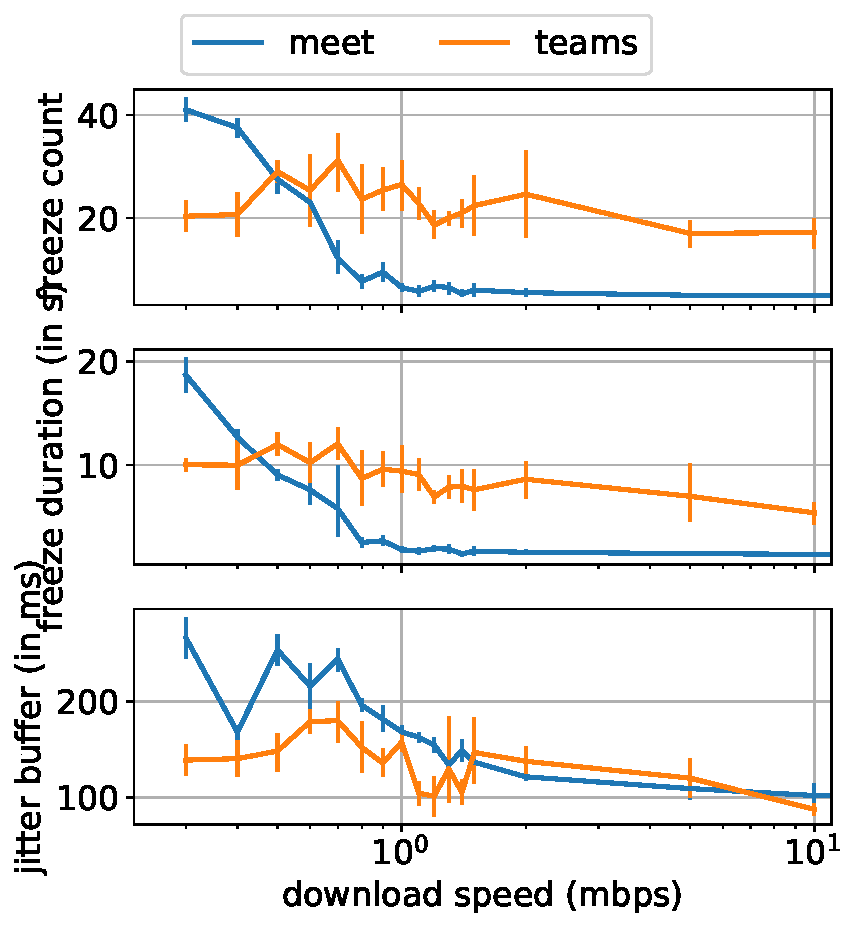
\includegraphics[width=0.35\textwidth,keepaspectratio]{figures/static/downlink_freeze_meet_teams.pdf}
    \caption{Downlink bandwidth and video freezes}
    \label{fig:downlink_freeze}
\end{figure}



\begin{figure}[]
    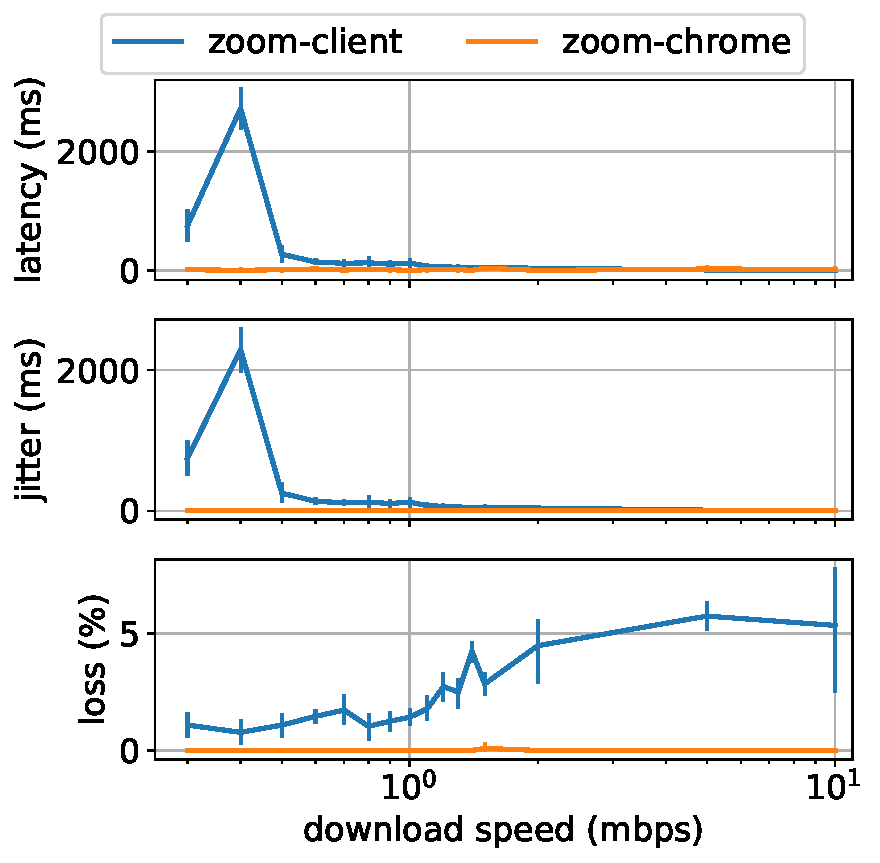
\includegraphics[width=0.35\textwidth,keepaspectratio]{figures/static/downlink_qos_zoom.pdf}
    \caption{Downlink bandwidth vs Zoom QoS. \jamie{It looks fishy, that zoom client latency and jitter are identical.  All data from browser seems to be zeroed out?}} 
    \label{fig:downlink_qos_zoom}
\end{figure}
\end{comment}